\chapter{Besoins fonctionnels}

\section{Modèle}
\subsection{Besoins}
Le modèle décrit les données manipulées par l'application. Dans un premier temps, notre modèle est celui des créatures. Par la suite nous utiliserons un modèle basé sur la bourse.

\begin{itemize}
 \item Priorité: importante.
 \item Justification: représente la base de notre application, l'algorithme génétique sera appliqué à ce modèle.\\
\end{itemize}




\subsection{Prototype papier}

\begin{figure}[H]
    \centering
    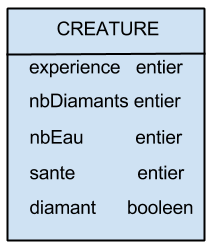
\includegraphics[width=0.3\textwidth]{./pictures/creature.png}
    \caption{Modèle de Creature}
\end{figure}



\section{Réseau de neurones}
\subsection{Besoins}
Le réseau de neurones permet à notre modèle de définir des actions en fonction des entrées (capteurs, status, etc). Il s'adapte suivant le modèle, c'est-à-dire au nombre et au type d'entrées.

\begin{itemize}
 \item Priorité: très importante.
 \item Justification: c'est le cerveau du modèle, il est adapté au fil des générations.\\
\end{itemize}



\subsection{Prototype papier}

\begin{figure}[H]
    \centering
    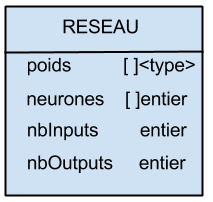
\includegraphics[width=0.3\textwidth]{./pictures/reseau.png}
    \caption{Réseau de neurones}
\end{figure}

\section{Algorithme génétique}
\subsection{Besoins}
L'algorithme génétique est notre fonction d'évaluation et de création de génération. Il est générique et s'adapte donc aussi au modèle.

\begin{itemize}
 \item Priorité: très importante.
 \item Justification: l'algorithme génétique est ce qui nous permet de faire évoluer (avec le réseau de neurones) le modèle durant plusieurs générations jusqu'à obtenir une solution, tendant vers l'optimale.\\
\end{itemize}
\subsection{Prototype papier}

\begin{figure}[H]
    \centering
    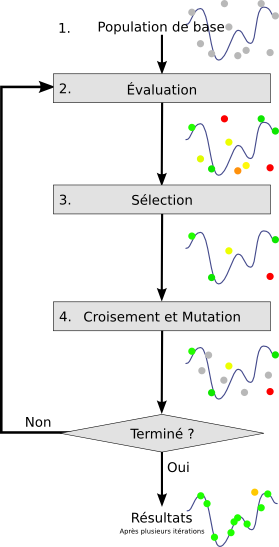
\includegraphics[width=0.4\textwidth]{./pictures/algorithme_genetique.png}
    \caption{Algorithme génétique}
\end{figure}


\section{Interface graphique}
\subsection{Besoins}
Description: nous avons besoin d'une méthode de visualisation claire et pertinente de nos résultats.
\begin{itemize}
 \item Priorité: importante.
 \item Justification: Afin d’avoir un résultat visuel nous avons besoin d’une interface qui va nous 
montrer en temps réel les agissement des créatures ainsi que leur évolution.\\
\end{itemize}


\subsection{Prototype papier}
\begin{figure}[H]
    \centering
    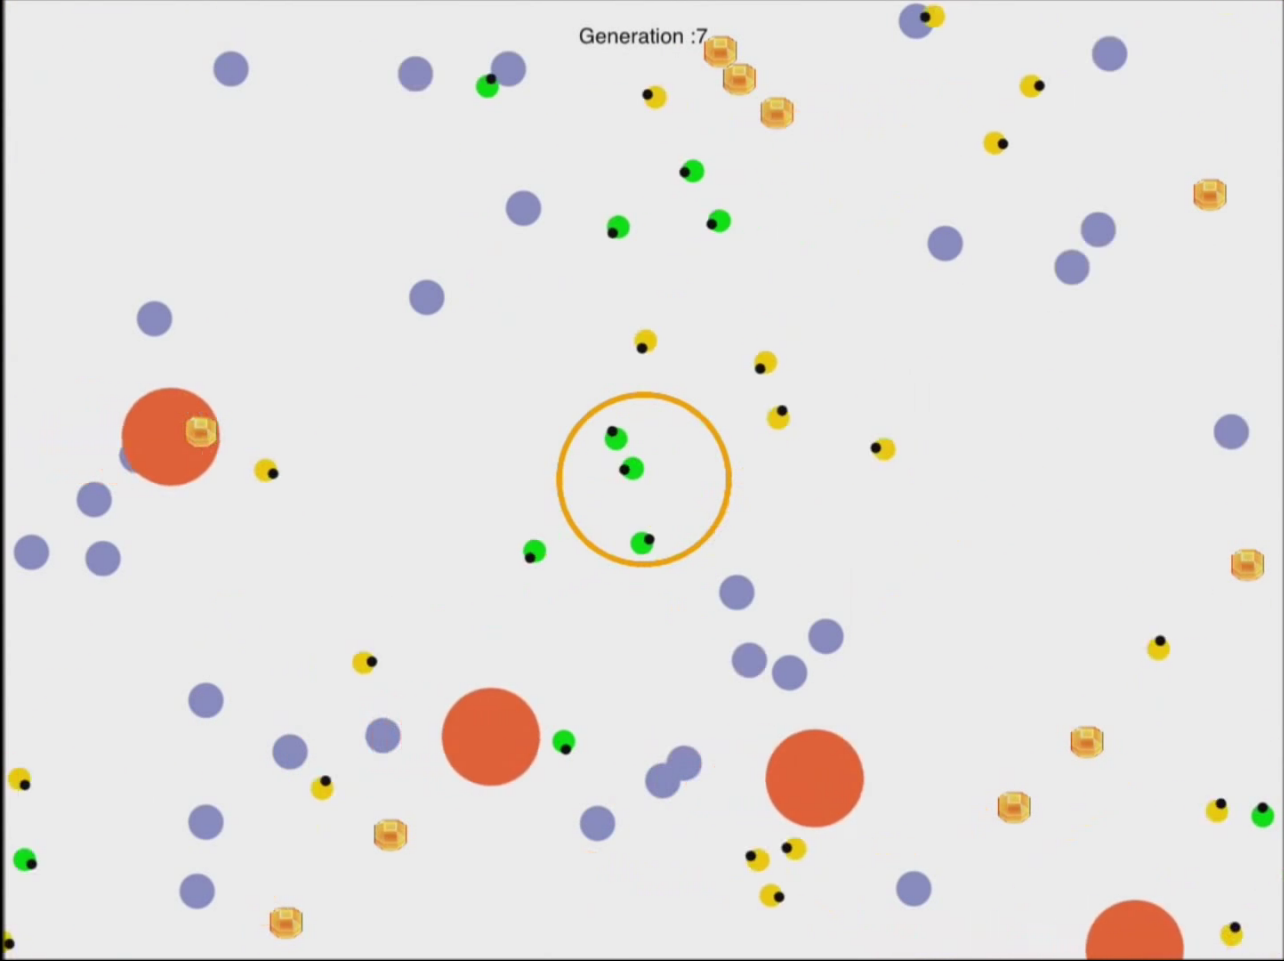
\includegraphics[width=0.8\textwidth]{./pictures/prototype.png}
    \caption{Interface}
    %\label{fig:awesome_image}
\end{figure}


\clearpage
